\section{Clock Delay}

While the clock signal for this system is accurate, students must force the
\ttt{OE} and \ttt{WE} pins to lag slightly behind the generation of individual
memory addresses.  This ensures that the memory address is correct and prevents
the memory address from changing during any single read or write operation.

The actual length of the delay is not critical, but it must be consistent
between clock cycles.  As such, the lab instructors provided a working method
with which the clock signal could be delayed.  By passing the clock through two
series boolean \ttt{AND} gates with the two input pins on each tied together, a
slight delay is introduced into the signal.  Figure~\ref{f:clock} shows such an
effect.
%
\begin{figure}[H]
\centering
	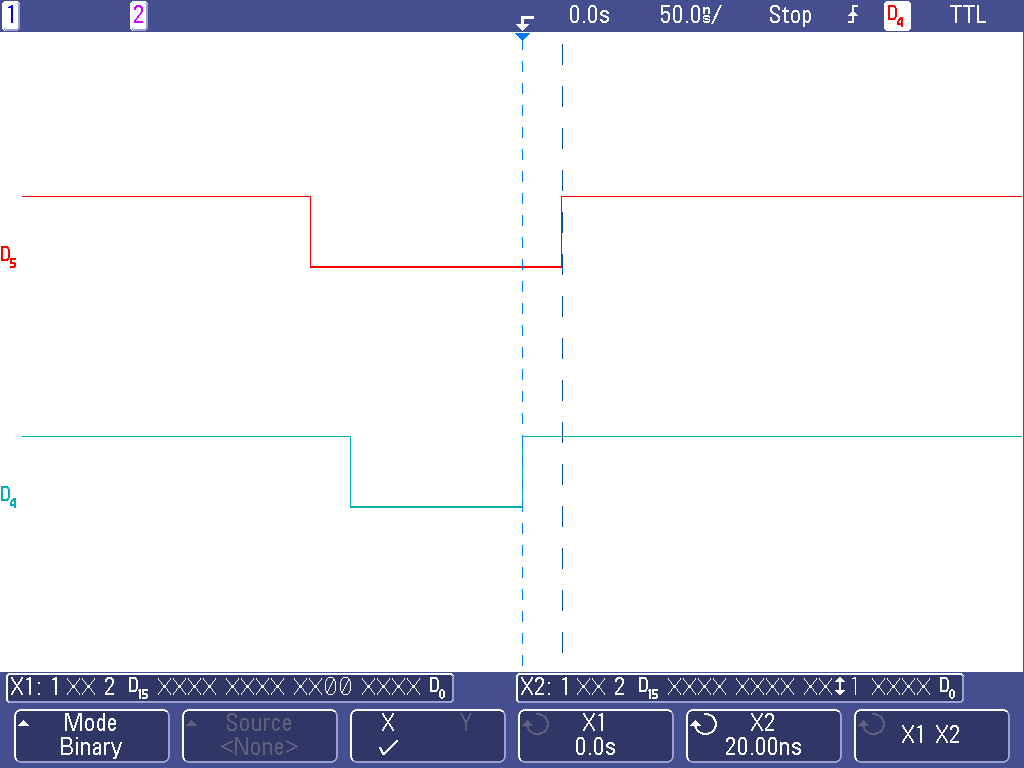
\includegraphics[width=.8\textwidth]{img/shot/and_delay.png}
	\parbox{.8\textwidth}{
	\caption[AND Gate Clock Delay]{Screenshot showing the effects of passing
	the clock signal through two \ttt{AND} gates.  Note that the lower signal
	was measured before entering the \ttt{AND} gates, whereas the upper signal
	was measured at the output of the second gate.  The delay, as measured by
	the oscilloscope, was~\SI{20}{\nano\second}.}
	\label{f:clock}}
\end{figure}
%
Figure~\ref{f:clock} shows the results of delaying the clock signal with two
\ttt{AND} gates from a 74LS08 quad \ttt{AND} IC.  The oscilloscope measured the
delay to be~\SI{20}{\nano\second} --- long enough to ensure that the generated
address has settled, but not so long that it causes the system to become
unstable.
